\chapter{Resultados}
\label{ch:Resultados}
\section{Processo de AM}
Esta seção descreve a realização do processo de AM, deste a coleta até a apresentação dos dados.
\subsection{Coleta}
A coleta dos dados foi realizada pelos pesquisadores Jorge Luiz (Engenheiro Eletricista) e Bruna da Silva (Fisioterapeuta), utilizanda o protocolo descrito no Apendice \ref{apendicetae}, o qual descreve detalhadamente todo o processo de coleta dos dados.

Os dados utilizados para a classificação, se refem a \textbf{Coleta 1 - Tremor de Repouso}, uma vez que esta apresentou os melhores resultados na classificação, já que as outras três coletas apresentavam um alto ruído que acabaram comprometendo os dados. A seguir um pequeno resumo sobre esta coleta.

Foram realizadas três coletas por colaborador, com duração de cinco segundos cada, a disposição dos eletrodos encontra-se no Apendice \ref{apendicetae}. Os dados do sinal foram aramazenadas através da utilização de 4 canais, sendo eles:
\begin{enumerate}
    \item \textbf{CH1}: Extensor radial do longo do carpo direito;
    \item \textbf{CH2}: Flexor superficial dos dedos direito;
    \item \textbf{CH3}: Extensor radial do longo do carpo esquerdo;
    \item \textbf{CH4}: Flexor superficial dos dedos esquerdo.
\end{enumerate}

Estes dados coletados em sEMG em cada canal, foram cedidos no formato \textit{edf}.

\subsection{Processamento dos dados}
Com os dados brutos iniciou-se a etapa de pré-processamento dos dados. Inicialmente utilizou-se como tecnica para a filtragem dos dados a Transformada rápida de Fourier (FFT), onde realizou-se testes nos quatro canais disponiveis, realizando um comparativo da acuracia com e sem a FFT, além de um comparativo sobre a acuracia entre os canais. 

Com relação aos dados obtidos em cada canal, como pode ser obsrvado na figura \ref{fcomparativo}, utilizando a fft obteve-se um bom resultado nos canais \textbf{CH1} com uma precisão de 78 e um resultado razoavel no \textbf{CH3} com precisão em 69.

Realizou-se também a aplicação de filtros de frequência, passa-banda, passa-baixa e passa-alta. Porém estes filtros diminuiram a acuracia obtida, como observado na figura \ref{comesemfiltro}, que exemplifica a matriz de confusão referente ao \textbf{CH1}, assim como normalizou-se os dados em diferentes escalas e do mesmo modo a acuracia caiu.

\begin{figure}[!htb]
	\centering
	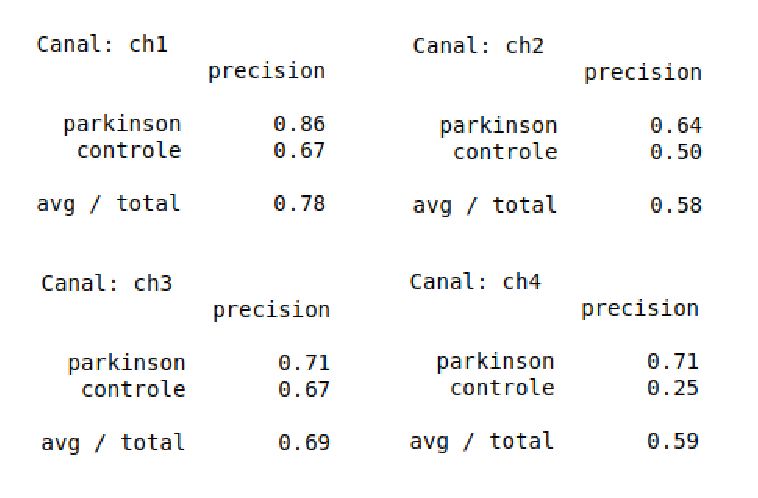
\includegraphics[width=0.8\textwidth]{figuras/fcomparativo.eps}
	\caption{Comparativo da precisão entre os canais, com a fft.}
	\label{fcomparativo}
\end{figure}

\begin{figure}[!htb]
	\centering
	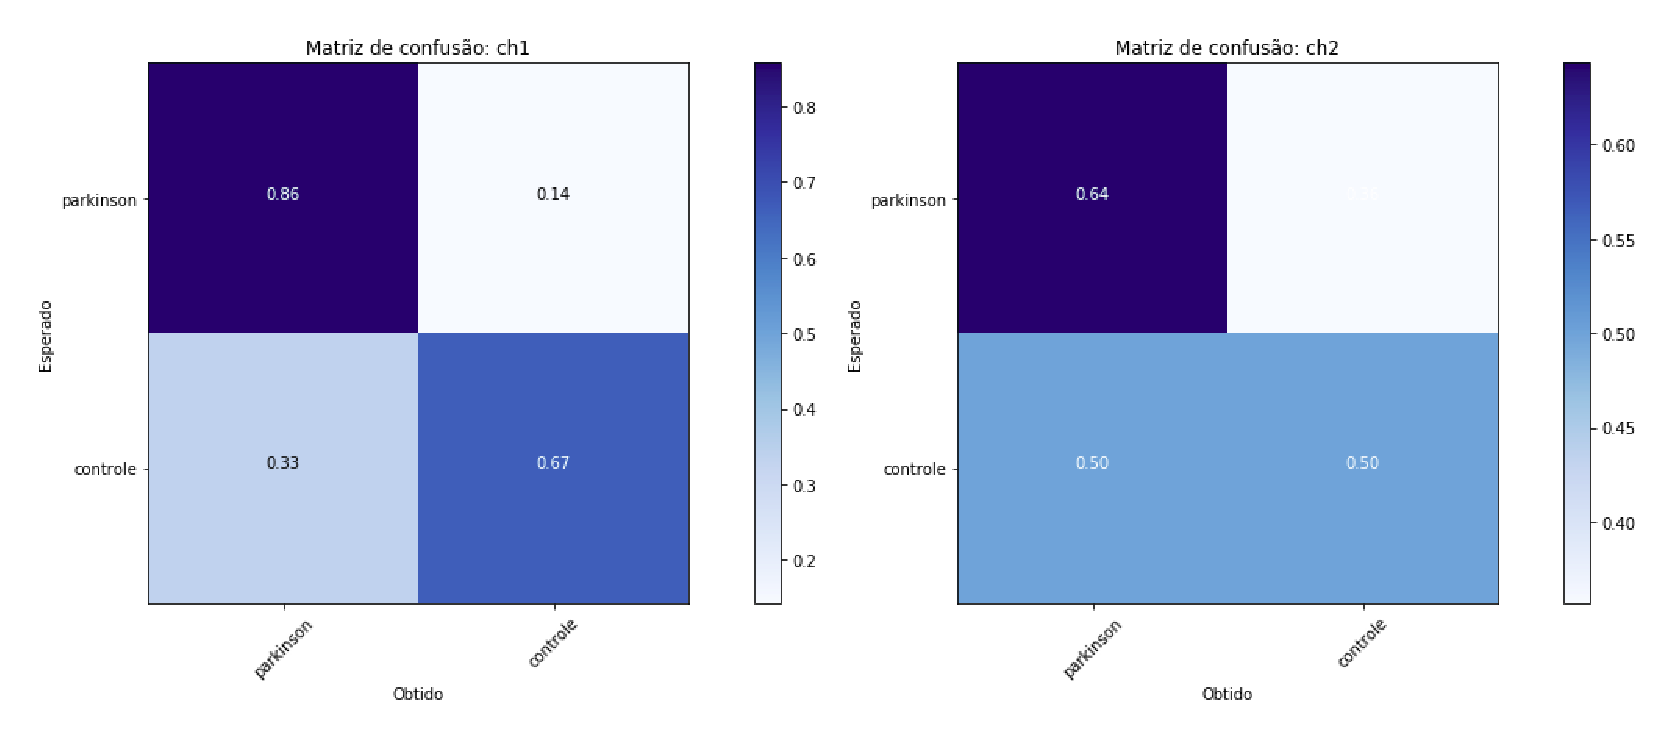
\includegraphics[width=1.1\textwidth]{figuras/CH12Comp.eps}
	\caption{Comparativo entre os canais 1 e 2, com a fft.}
	\label{fcomparativo}
\end{figure}

\begin{figure}[!htb]
	\centering
	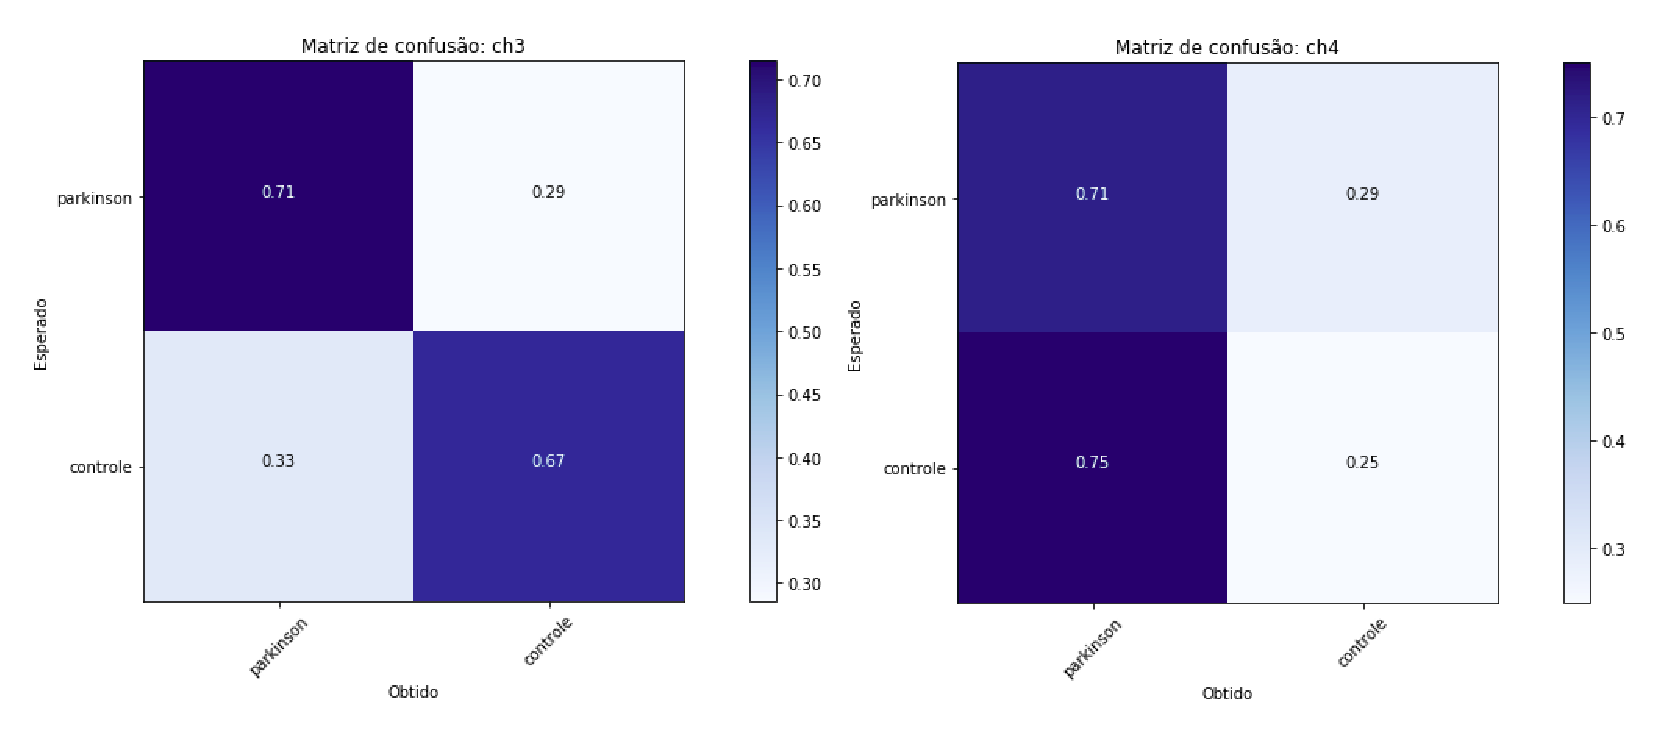
\includegraphics[width=1.1\textwidth]{figuras/CH34Comp.eps}
	\caption{Comparativo entre os canais 3 e 4, com a fft.}
	\label{fcomparativo}
\end{figure}


\begin{figure}[!htb]
	\centering
	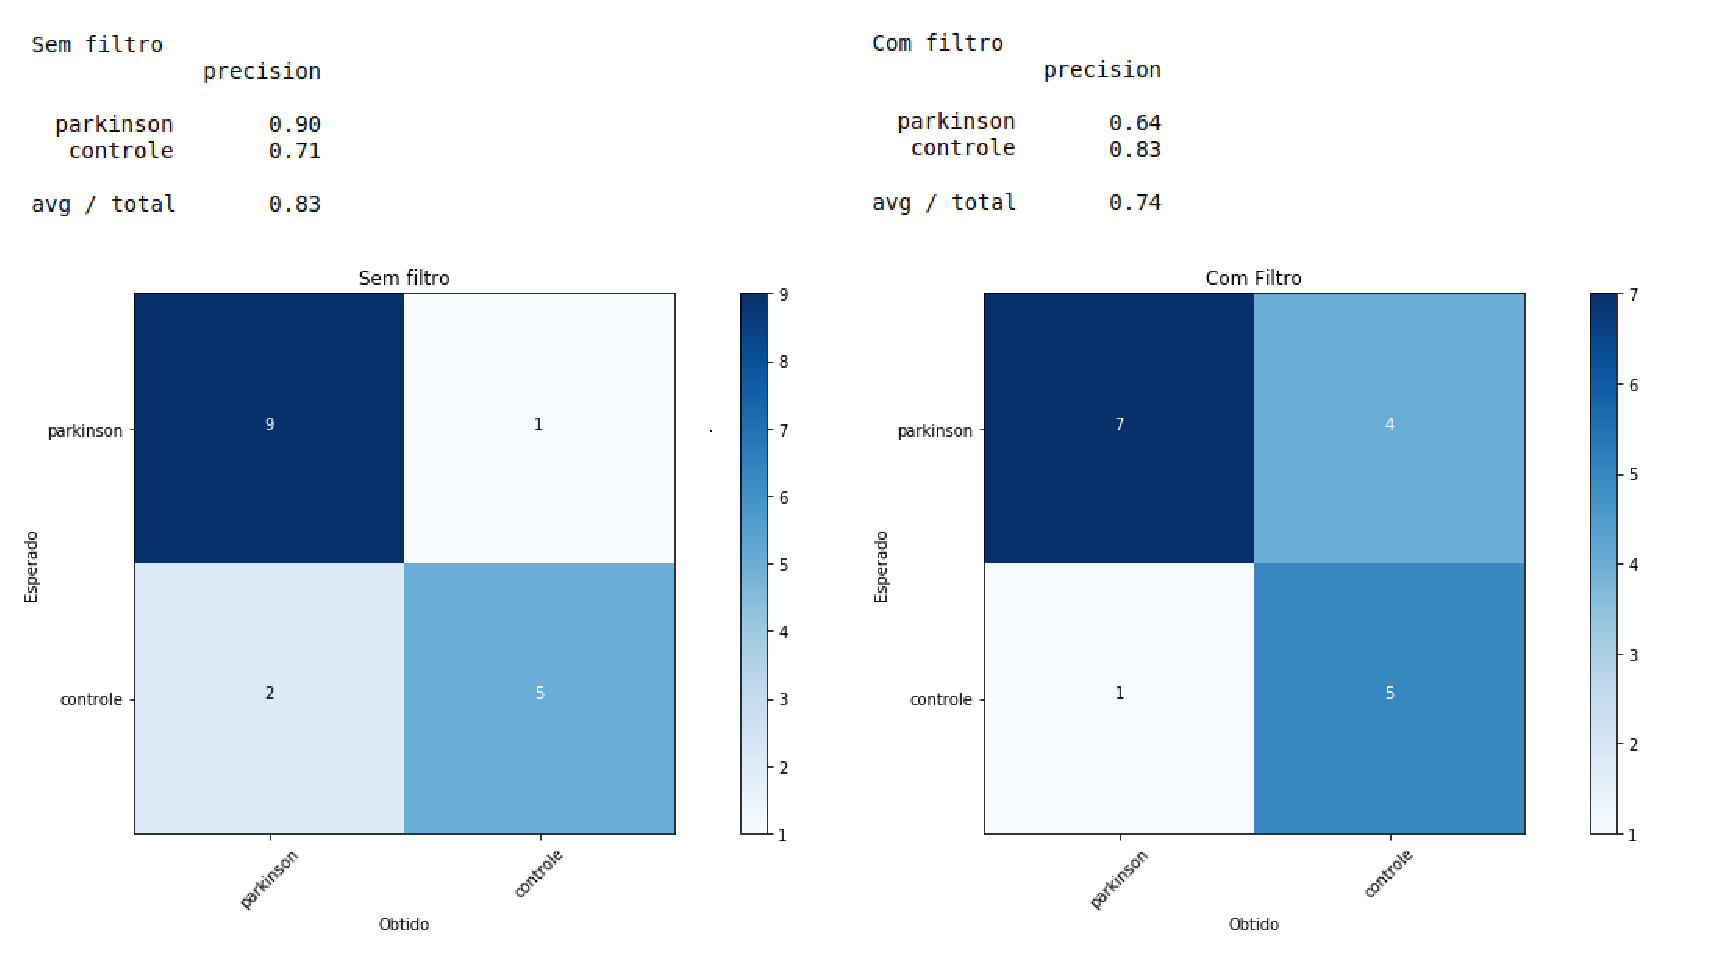
\includegraphics[width=1.1\textwidth]{figuras/filtroComp.eps}
	\caption{Matriz de confusão com e sem filtro do \textbf{Ch1}.}
	\label{comesemfiltro}
\end{figure}

Também realizou-se a classificação utilizando todos os canais ao mesmo tempo, porém o resultado foi insatisfatorio.

Outra técnica de selecão de feature utilizada foi a PCA ou Análise de componentes principais, com a utilização desta tecnica obteve-se uma leve melhora na acuracia, como pode ser observado na figura \ref{pcavalidator}, a qual utilizou-se o \textit{k-fold cross-validator} para verificar a precisão real do modelo.

Como pode ser observado na figura \ref{pcavalidator}, com o auxilio do k-fold, pode-se inferir que o Random Forest possui uma precisão superior ao SVM, além de que o PCA aumenta a acuracia consideravelmente do modelo.

\begin{figure}[!htb]
	\centering
	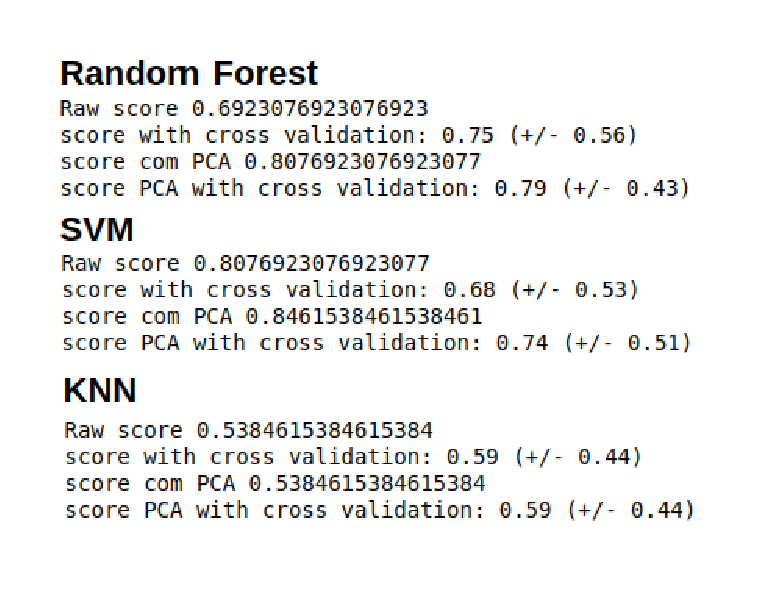
\includegraphics[width=1.1\textwidth]{figuras/modeloComp.eps}
	\caption{Matriz de confusão com e sem filtro do canal 1.}
	\label{pcavalidator}
\end{figure}

Finalizando a etapa de pré-processamento dos dados, concluiu-se que a utilização da FFT com o PCA mostrou-se a melhor combinação para obtermos os melhores resultados, com o \textit{Random Forest} levemente superior ao SVM e o KNN, com as respectivas precisões.

\subsection{Apresentar dos dados}

\section{Solução de software}
\subsection{Arquitetura}
O documento de Arquitetura encontra-se no anexo \ref{adoarquitetura} na página \pageref{adoarquitetura}.

\subsection{Visão}
O documento de Visão encontra-se no anexo \ref{adocvisao} na página \pageref{adocvisao}.

\subsection{Produto}
Os detalhes referentes a construção do produto encontram-se descritos no documento de Visão \ref{adocvisao} e no documento de Arquitetura \ref{adoarquitetura}, a seguir as telas do sistema.

Pagina inicial

\begin{figure}[!htb]
    \centering
    \includegraphics[width=0.9\textwidth]{figuras/produto/home.eps}
    \caption{Diagrama de pacotes}
    \label{fighome}
\end{figure}

\begin{figure}[!htb]
    \centering
    \includegraphics[width=0.9\textwidth]{figuras/produto/cadastro.eps}
    \caption{Cadastro das pacientes}
    \label{figcadastro}
\end{figure}

% \begin{figure}[!htb]
%     \centering
%     \includegraphics[width=1\textwidth]{figuras/produto/editar.eps}
%     \caption{Editar dados dos pacientes}
%     \label{figeditar}
% \end{figure}

% \begin{figure}[!htb]
%     \centering
%     \includegraphics[width=1\textwidth]{figuras/produto/avaliar.eps}
%     \caption{Avaliar pacientes}
%     \label{figavaliar}
% \end{figure}

% \begin{figure}[!htb]
%     \centering
%     \includegraphics[width=1\textwidth]{figuras/produto/pesquisar.eps}
%     \caption{Pesquisar itens pelas colunas}
%     \label{figpesquisar}
% \end{figure}


% \begin{figure}[!htb]
%     \centering
%     \includegraphics[width=1\textwidth]{figuras/produto/outrasop.eps}
%     \caption{Downloand da tabela, impressão e exibir colunas}
%     \label{figoutrasop}
% \end{figure}